\section{簡介}
由於模型過於複雜,對於解碼器而言所產生的句子容易出現重複的字,並不明顯合乎語言模型(Language Model)的句子,為了解決這個問題,我們打算分開解碼器模型的部分,事先訓練好一個解碼器,以減少重複字出線的狀況。
\section{變分遞迴式自動編碼器}
我們採用隨插即用(Plug and Play)\cite{nguyen2016plug} 的概念,我們先針對在解碼器的部分,我們採用預訓練(Pre-train)的方法。首先訓練一個自動編碼器(AutoEncoder),此自動編碼器結合遞迴式類神經網路 \cite{bowman2015generating} 和變分(Variational)的方法,稱為變分遞迴式自動編碼器(Variational Recurrent AutoEndoder),再將訓練好的自動編碼器只取其解碼器的模型,接回專注式記憶編碼解碼器,來達到更好的成效。
\begin{figure}[h]
    \centering
    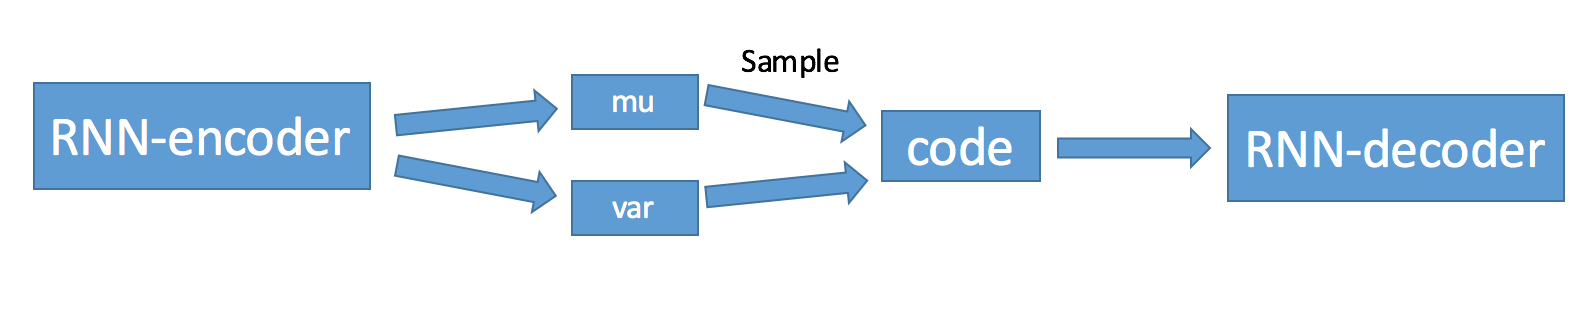
\includegraphics[scale=0.52]{images/chap5_vrae.png}
    \caption{變分遞迴式自動編碼器}\label{fig:vrae}
\end{figure}
\subsection{遞迴式自動編碼器}
遞迴式自動編碼器與自動編碼器的概念相似,差別是在潛在向量(Latent Vector)的編碼方式是透過遞迴式類神經網路來取得,也用遞迴式網路來重建句子。
\subsection{變分機制}
我們對遞迴式自動編碼器的部分加入了變分機制,如圖(\ref{fig:vrae}),編碼器降維到一個潛在空間(Latent Space)$q_\theta(z|x)$ ,其中 $\theta$ 代表編碼器的參數(Parameter)。 編碼後的結果去得到平均值 $\mu$(Mean)與變異數 $\sigma$(Variance),並能得到基於編碼器所形成的分佈 (Distribution)。
之後在用 $q_\theta(z|x)$ 來取樣(Sample)出潛在變量 $z$(Latent Variable),如式子(\ref{function:sample})。
%$p_\phi(x|z)$而這個分佈的平均值是 0 ,而變異數是 1 ,如式子 \ref{function:prob},並由此分佈來取樣(Sampled)出潛在變量(Latent Variable),如式子\ref{function:sample} ,當作解碼器的初始狀態(Initial State)。
\begin{equation}
    z = \mu + \sigma \odot \epsilon \label{function:sample}
\end{equation}
其中 $\epsilon \sim Normal(0,1)$ 。

以潛在變量當作解碼器的初始狀態,以此來重建(Reconstruct)回原來的句子,在此以 $p_\phi(x|z)$ 表示,$\phi$ 代表解碼器的參數。
%\begin{equation}
%    q_\theta(z|x) p(z)
%    p_\phi(x|z)
%    \label{function:prob}
%\end{equation}
這時候,問題就變成要讓 $q_\theta(z|x)$ 接近高斯分佈(Gaussian Distribution)以及能重建回輸入的準確率。要讓此分佈趨近高斯分佈,我們靠得是克雷散度(Kullback–Leibler Divergence)。
\subsection{克雷散度}
克雷散度是用以衡量兩組機率分佈的距離,值越大則代表兩組分佈越不相似。我們試著衡量編碼器的分佈 $q_\theta(z|x)$ 與 $p(z)$ ,衡量兩者之間有多相似,如式子(\ref{function:KL})。
\begin{equation}
    -D_{KL}(q_\phi(z|x)|| p_\theta(z) ) = \frac{1}{2} \sum(1+\log(\sigma^2) - \mu^2 - \sigma^2)
    \label{function:KL}
\end{equation}
其中$p(z)$ 在變分自動編碼器裡為標準常態分佈(Standard Normal Distribution)。
\subsection{損失函數}
整個變分遞迴式自動編碼器模型的損失函數,是由一般遞迴式自編碼器加上正規化所組成,如式子(\ref{function:vrae_loss})。
\begin{equation}
    C(\theta, \phi) = -E_{q_{\theta}}[\log p_\phi(x|z)] + KL(q_\theta(z|x) \| p(z))
    \label{function:vrae_loss}
\end{equation}
第一項代表重建損失(Reconstruct Loss),若無法完整重建句子,則該值會很大。
而第二項則代表編碼器所產生的潛在變量 $z$ 與標準常態分佈之間的差距,該項代表的意義是為了讓潛在變量保持夠多樣(Diverse),例如代表兩個相似意思的句子,在潛在空間裡應該要相近。在此處,我們給予克雷散度一個最低限度,因為 KL 項相較第一項而言容易趨近於 0 ,且容易訓練,但我們最主要的目的是為了重建完整的句子,因而在此處我們給他最低的 KL 值 4 ,讓整個損失函數不置於過度貼合。
%z∼qϕ(z|x)
%$z ~ N(z_{mean}, np.exp(z_{log_{sigma}})^{2})$

%qϕ(z|x) , x̃ ∼pθ(x|z)
%KL divergence
%% Lower bound KL: 4
%difficulty
%% overfit
%variational
\section{實驗結果與討論}
\subsection{變分遞迴式自動編碼器實驗}
%TODO
在變分遞迴式自動編碼器的結果,我們測試重建之結果,在「Yes」、「No」、「approximately number\_0 per year」等的這種簡短的句子中,都能準確的重建出句子,但若是較長的句子,如「by an infection of oil glands in the eyelid」,仍不是特別理想,僅只能重建成「a infection of infection」。或許若是有足夠的訓練資料,會有更好的表現。
\subsection{問答系統模型結果}
在此,我們對訓練好的解碼器,測試與原先的模型比較,以及對解碼器微調(Fine Tune)後的結果來分析。如表 \ref{table:vrae} 所見,我們可發現,在無微調前,直接使用預先訓練好之解碼器,所得到的結果比最初的模型結果還差;然而,若是把解碼器跟著專注式記憶編碼解碼器一起進行訓練、微調,能夠使我們的模型更加進步。%能得到我們目前模型最好的結果。
\begin{table}[ht]
    \caption{採用變分遞迴式自動編碼器之結果} 
    \label{table:vrae}
    \centering
    \begin{tabular}{|l|l|}
        \hline
        模型架構 & ROUGE\\
        \hline
        原始模型 & 33.95\%\\
        \hline
        無微調 & 15.56\%\\%1974768\\
        \hline
        微調 & 34.32\%\\%\\
        \hline
    \end{tabular}
\end{table}
% VRAE loss
%fine tuning or not
\section{本章總結}
隨插即用的方法在生成對抗網路(GAN, Generative Adversarial Network)被使用,而我們將此概念移植至我們的實驗當中,亦能獲得進步,代表預先訓練好一個模型,降低模型訓練的難度,利用隨插即用的技術,能夠讓整體模型更好訓練,亦有更好的表現。%故若是能有更好的解碼器,應該會有更好的結果。
